\documentclass{article}
\usepackage{graphicx}
\usepackage[T2A]{fontenc}
\usepackage[utf8]{inputenc}
\usepackage[english,russian]{babel}
\usepackage{wrapfig} %обтекание картинки текстом
\usepackage{hyphenat} %для переноса слов
\usepackage{float} %чтобы картинка двигалась нормально с текстом
\usepackage{amsmath}
\usepackage{amssymb}
\usepackage{enumitem}
\hyphenation{о-пе-ра-ци-он-ны-ми}
\hyphenation{со-бы-тий-на-я}
\hyphenation{иг-ро-во-му}
\hyphenation{вза-и-мо-дей-стви-и}
\hyphenation{вза-и-мо-дей-стви-я}
\hyphenation{ис-поль-зу-ют}
\hyphenation{на-по-ми-на-ет}
\hyphenation{ко-то-ры-е}
\hyphenation{раз-лич-ны-ми}
\hyphenation{заб-ро-шен-ный}
\hyphenation{рас-се-яв-шие-ся}

\title{Диздок}
\author{}
\date{Ноябрь 2024}

\begin{document}

\maketitle

\tableofcontents

\newpage
\section{Введение}
Над созданием игры работали 6 человек: \\
Екатерина Наумова и Анастасия Веренинова, отвечающие за визуальную часть
проекта,\\
Егор Косых, Андрей Булычев и Иван Гайфиев, ответственные за разработку кода,\\
и Анна Малянова, оказывающая поддержку остальным участникам.

Идея сундука-обманки вдохновлена Мимиком из "Подземелье Вкусностей" Рёко Куи, монстром который маскировался под сундуки с золотом.

\section{Концепция}

\subsection{Введение}
Данная игра погружает пользователя в мир тёмного фэнтези с атмосферой 
средневековья, где его главной целью является исследование обширных 
и опасных локаций, сражения с боссами и, в конечном счёте, разгадка 
тайны игрового мира, в котором он оказался. \par Игра ориентирована на любителей 
фэнтези и мрачного лора в возрасте от 12 лет и старше. \par Одной из особенностей 
геймплея являются уникальные механики и событийная система, которая не 
даёт игроку заскучать благодаря случайным событиям, происходящим с его 
персонажем. \par Игра предназначена для запуска на персональных компьютерах 
с операционными системами Windows или macOS. \par Предпосылкой для её создания стали 
популярность жанра и любовь авторов к разработке увлекательных игр.

\subsection{Жанр и аудитория}
Игра представляет собой 2D-соулслайк в средневековом дарк-фэнтези стиле. Это жанр, который акцентирует внимание на сложных боях, исследовании обширных и атмосферных локаций. Игроки будут сталкиваться с различными врагами, включая монстров и боссов, требующими стратегического подхода и мастерства в бою. Элементы RPG, такие как прокачка персонажа, сбор предметов и взаимодействие с окружающим миром, придают глубину игровому процессу.\\[2mm] \parЦелевая аудитория игры — игроки в возрасте от 12 до 18 лет. Эта группа включает как опытных геймеров, знакомых с жанром соулслайков, так и новых игроков, ищущих интересный сюжет.\\[2mm] \parИгра будет позиционироваться как сложный и атмосферный проект, который предлагает игрокам уникальный опыт в исследовании мрачного фэнтезийного мира.  \\[2mm] \parПоэтому, игра будет не только развлекательной, но и предоставит игрокам возможность погрузиться в атмосферный и сложный мир дарк-фэнтези, где каждая локация отличается завораживающим окружением.

\subsection{Основные особенности игры}
То, что выделяет эту игру на фоне других в данном жанре - уникальные механики и система событий в игровом мире, которые не дадут игроку стоять на месте и расслабляться. События могут происходить случайно либо после определенного взаимодействия игрока с окружением. \\[2mm] \parТуман - случайное событие в локациях открытой местности (не внутри помещений), блокирует видимость игрока если рядом нет источника света. Нахождение в тумане более 5 секунд вызывает галлюцинации, имитирующие звуки врагов-монстров и горящие глаза. Туман наносит периодический урон, иллюзорным врагам нельзя нанеси урон. Чтобы избежать вред события, необходимо найти источник света или иметь его экипированным. \\[2mm] \parСундуки-обманки - предмет расположенный на локации, внешне напоминает обычный сундук, но отличается пятном на крышке. При нахождении рядом с данным предметом  некоторый промежуток времени (без взаимодействия) сундук-обманка показывает зубы, что позволяет вычислить его. При взаимодействии с сундуком-обманкой игрок теряет определенное количество здоровье и имеет риск потери случайного предмета из экипировки. \\[2mm] 

\subsection{Описание игры}
Игроку предстоит исследовать обширные и опасные замки и подземелья, сражаясь с монстрами и боссами, чтобы разгадать тайну мира, в котором он очутился. Сюжет завязан на раскрытии на тропе амнезии, где игрок собирает воспоминания по крупицам, исследуя локации, побеждая монстров.\\[2mm]\par
Игровая завязка строится на том, что игрок просыпается в заброшенном замке, поглощенном таинственным туманом. Он/она ничего не помнит, кроме смутных обрывков воспоминаний, связанных с этим местом. Вокруг него – темные залы, освещенные факелами и разбросанные книги, и обрывки записок. Каждая записка содержит фрагменты истории замка и дает намеки на прошлое главного героя, его связь с этим местом, предостережения о возможных будущих опасностях. Ему/ей предстоит исследовать заброшенный замок, чтобы собрать информацию о том, что произошло из записок и с рассказов выживших. По ходу исследования главный герой сталкивается с живыми скелетами, теневыми существами и различными ловушками, которые активируются по мере его продвижения по локации. В записках можно узнать, что в замке проводились магические эксперименты, связанные с древним артефактом Бездны, который пробудил и впустил в мир темные силы. Одна из записок упоминает некого персонажа, который может помочь нашему герою. Следующая цель найти способ покинуть проклятый замок,  разыскать убежище, чтобы спрятаться на первое время. Покинув замок, игрок сталкивается с загадочным незнакомцем, который говорит, что знает, как остановить тьму, распространившуюся по королевству. Незнакомец сообщает, что это королевство было захвачено злыми силами, которые используют артефакт для подчинения мертвых. Игроку придется отправиться в путешествие по землям королевства, чтобы уничтожить рассеявшиеся силы зла, сразиться с "хранителями" и собрать части артефакта, чтобы в конечном итоге добраться до Сердца Бездны. В итоге герою предстоит пройти 4 локации разной сложности и их боссов, чтобы победить зло и освободить королевство от заклятия. Однако, появившийся из ниоткуда, незнакомец намекает, что не все угрозы уничтожены, а что же будет дальше герою придется узнать в следующих частях..


\subsection{Предпосылки создания}
Хотелось бы начать с описания факта популярности игр в современном мире. Люди проводят так свободное время, отдыхают, находят друзей в онлайн играх. Также как и большинство, участники этого проекта являются фанатами игр. Именно поэтому мы решили создать игру, которая будет интересна именно нам и также другим любителям игр. 

Как уже было замечено, наша игра представлена в стиле souls-like в 2D формате. В современном мире этот стиль занимает высокие позиции по популярности, поэтому нас заинтересовало сделать что-то новое именно в этом жанре. Идеально отлаженный игровой процесс, сочетающийся с высокой сложностью, внутриигровое социальное взаимодействие, огромный потенциал для обсуждения, таинственный и захватывающий мир, который требует тщательного изучения и исследования - все это основные черты нашей игры. 

Безусловно наш проект может быть похож на другие в этом жанре, хотя и не имеет привязке к уже созданным вселенным из книг и фильмов, но также включает в себя много уникальных компонентов и идей (локации, тайны для разгадки и многое другое). 

\subsection{Платформа}

\begin{tabular}{|c|cc|}
\hline

Требования               & \multicolumn{1}{c|}{Минимальные}            &
Рекомендуемые         \\ \hline
Операционная система     & \multicolumn{2}{c|}{Windows (64 bit)}                               \\ \hline
Процессор                & \multicolumn{1}{c|}{Intel Core 2 Duo E8400} & Intel Core i3         \\ \hline
ОЗУ                      & \multicolumn{1}{c|}{4 GB}                   & 6 GB                  \\ \hline
CD-ROM привод            & \multicolumn{2}{c|}{Не требуется}                                   \\ \hline
Свободное место на диске & \multicolumn{2}{c|}{4 GB}                                           \\ \hline
Видеокарта               & \multicolumn{1}{c|}{NVIDIA GeForce GT 520}  & NVIDIA GeForce GT 710 \\ \hline
Звуковая карта           & \multicolumn{2}{c|}{Любая встроенная}                               \\ \hline
Управление               & \multicolumn{2}{c|}{Геймпад, клавиатура}                            \\ \hline
\end{tabular}
\\[10mm]

\begin{tabular}{|c|cc|}
\hline
Требования               & \multicolumn{1}{c|}{Минимальные}            & Рекомендуемые        \\ \hline
Операционная система     & \multicolumn{2}{c|}{MacOS (64 bit)}                                \\ \hline
Процессор                & \multicolumn{1}{c|}{Intel Core i3}          & Intel Core i3 2.4GHz \\ \hline
ОЗУ                      & \multicolumn{1}{c|}{4 GB}                   & 6 GB                 \\ \hline
CD-ROM привод            & \multicolumn{2}{c|}{Не требуется}                                  \\ \hline
Свободное место на диске & \multicolumn{2}{c|}{4 GB}                                          \\ \hline
Видеокарта               & \multicolumn{1}{c|}{Nvidia GeForce GT 640M} & GeForce GTX 570      \\ \hline
Звуковая карта           & \multicolumn{2}{c|}{Любая встроенная}                              \\ \hline
Управление               & \multicolumn{2}{c|}{Геймпад, клавиатура}                           \\ \hline
\end{tabular}


\section{Функциональная спецификация}

\subsection{Принципы игры}

\subsubsection{Суть игрового процесса}
\par  Суть игрового процесса подразделяется на следующие основные части:
\begin{itemize}
\item \textbf{Исследование мира} \par  Игроки погружаются в обширный мрачный мир, наполненный секретами, скрытыми путями и уникальными локациями. Каждый уголок замков и подземелий может содержать ценные предметы, загадки или неожиданные встречи с NPC. Чувство открытия и исследования возникает, когда игроки находят новые области, раскрывают историю мира и взаимодействуют с его обитателями. 
\item \textbf{Настройка персонажа}  Игроки могут настраивать и видоизменять своих персонажей, опираясь на свои предпочтения и вкус. Это создает чувство прогресса и индивидуальности, а также удовлетворение от достижения новых уровней, открытия новых способностей и создания уникального персонажа. \item\textbf{Лут и предметы}  \par  Игроки находят разнообразные предметы, которые могут быть использованы для улучшения снаряжения или создания новых предметов. Лут может быть случайным или находиться в сундуках, что добавляет элемент неожиданности. Радость от нахождения редких предметов и возможности их использования для улучшения боевых навыков делает игру еще более увлекательной.\item\textbf{Механики боя}  \par  В игре используются механики уклонения, блокировки и контратак, что делает каждую битву захватывающей и непредсказуемой. Игроки могут экспериментировать с разными стилями боя в зависимости от выбранного класса, получая удовольствие от мастерства в бою и понимания механик врагов, что позволяет чувствовать себя настоящими героями. \item\textbf{Взаимодействие с NPC} Взаимодействие с NPC заключается в решении головоломок и выполнении квестов, добавляющих глубину в игровой процесс. Игроки могут принимать решения, которые влияют на ход событий и мир вокруг них, что приносит удовольствие от вовлеченности в сюжет и возможности влиять на развитие истории.\item\textbf{Удовольствие от преодоления трудностей} \par  Удовольствие от продвижения по сюжету получается посредством преодоления трудностей и решением стоящих перед игроками задач. Победы над сильными врагами и завершения сложных заданий способны особенно сильно отозваться в душе пользователей. Также, возможность настраивать персонажа под свой стиль игры позволяет каждому создать показать свой вторческий гений. Захватывающая история и богатый мир создают желание как можно глубже погрузиться в суть происходящего.
\end{itemize}

\subsubsection{Ход игры и сюжет}
\paragraph{Типичный сеанс игры: }
\subparagraph{1. Запуск игры и выбор персонажа \\}
Игрок запускает игру, попадает в главное меню, где выбирает класс персонажа: мечник или маг. После этого ему предлагается настроить внешний вид героя и начать приключение. 
\subparagraph{2. Начало приключения: Заброшенный замок \\}
Персонаж приходит в себя на полу в одном из залов старого замка, освещенного тлеющими факелами. Камера плавно облетает локацию, демонстрируя атмосферу. Игрок получает первые подсказки управления и начинает исследовать окрестности.
\begin{itemize}
\item[*] Собирает первые записки, узнает об экспериментах с магическим артефактом.
Сталкивается с первыми врагами: скелетами и тенями, учится использовать базовые атаки и уклонения.
\item[*] Находит сейв-зону – старую часовню, где можно восстановить здоровье и сохранить прогресс.
\end{itemize}
\subparagraph{3. Встреча с Незнакомцем \\}
Покинув замок через тайный проход, игрок встречает загадочного Незнакомца у костра. Тот объясняет, что для победы над тьмой нужно собрать три части артефакта. Игрок получает карту с отмеченными основными локациями. \\
\subparagraph{4. Путешествие по первым локациям \\}
\begin{itemize}
\item[*] Проклятый Лес: Игрок пробирается через густую чащу, постоянно сталкиваясь с волками и пауками. Здесь игрок впервые получает задание решить головоломку с часовым механизмом, чтобы открыть путь к боссу.
1. Бой с Древним Оборотнем: Бой требует стратегического подхода – игрок использует ловушки, чтобы ослабить врага. \\
2. Награда: Первая часть артефакта и светящийся амулет, который помогает видеть в темноте.
\item[*] Скалы Пепельного Крика: Путь через старые горные туннели. Игрок сталкивается с ловушками и сильными духами. Необходимо активировать защитные обряды, чтобы разрушить барьеры.
1. Бой с Тенью Некроманта: Враг использует заклинания и вызывает миньонов. Игрок должен разрушить кристаллы, чтобы ослабить его защиту. \\
2. Награда: Вторая часть артефакта и новое заклинание или усиление оружия. \\
\end{itemize}
\subparagraph{5. Развитие персонажа}
Между миссиями игрок может:
\begin{itemize}
\item[*] Прокачивать навыки: Улучшать атаку, здоровье и магические способности.
\item[*] Оружие и доспехи: Улучшать или находить редкое снаряжение в сундуках.
\item[*] Поиск артефактов: Некоторые артефакты дают пассивные бонусы, например, увеличение скорости или защиту от яда.
\end{itemize}
\subparagraph{6. Концовка сеанса \\}
В определенных точках (сейв-зоны) игрок может завершить сеанс, сохранив весь прогресс. При следующем запуске игра предложит продолжить с последнего сохранения. \\
\paragraph{Лор и атмосфера мира \\}
Действие происходит в мире, который долгое время существовал в гармонии, пока маги замка не пробудили Сердце Бездны – могущественный артефакт, способный управлять жизнью и смертью. Силы тьмы поглотили все земли вокруг, превратив некогда процветающее королевство в пустошь, населенную монстрами и нежитью.
\begin{itemize}
\item[*] Проклятый Лес был некогда священной рощей, но после экспериментов стал местом вечной ночи.
\item[*] Скалы Пепельного Крика — это древнее святилище, использовавшееся для обрядов некромантов.
\item[*] Подземелья Бездны были тюрьмой для самых опасных существ, но теперь превратились в логово тьмы.
\end{itemize}
Каждая зона наполнена уникальной историей, записками и визуальными деталями, погружающими игрока в мир, полный тайн и угроз.


\subsection{Физическая модель}
Физическая модель игры будет реалистично симулировать взаимодействие объектов и персонажей в 2D-пространстве, создавая ощущение живого, динамичного мира. Основное внимание уделяется перемещениям, боевым действиям и взаимодействию с окружением. Ниже описаны ключевые аспекты физической модели:

\subsubsection{Перемещения}

\begin{itemize}
    \item \textbf{Гравитация:} Все персонажи и объекты подчиняются закону гравитации, что определяет их падение с высоты и скорость приземления. Например, персонаж будет набирать скорость при падении, а при столкновении с поверхностью получит урон в зависимости от высоты.
    \item \textbf{Скорость передвижения:} У каждого класса персонажей будет своя базовая скорость передвижения, которая может быть изменена с помощью экипировки или специальных предметов.
    \item \textbf{Прыжки:} Игроки смогут совершать прыжки фиксированной высоты (которая может измениться с помощью возможных улучшений)
    \item \textbf{Лазание:} С помощью специальных предметов игрок сможет взаимодействовать со стенами для лазания по ним.
    \item \textbf{Полеты:} Некоторые предметы позволят временно игнорировать гравитацию, что откроет новые возможности для исследования.
\end{itemize}

\subsubsection{Боевые действия}

\begin{itemize}
    \item \textbf{Удары ближнего боя:} Каждое оружие имеет радиус и скорость атаки. Масса оружия влияет на его инерцию: тяжёлое оружие наносит больше урона, но требует больше времени для замаха.
    \item \textbf{Дальние атаки:} Магические снаряды имеют фиксированную скорость и дальность. Они могут быть заблокированы препятствиями или щитом.
    \item \textbf{Урон:} Урон рассчитывается по формуле, учитывающей базовый урон оружия или заклинания, уровень персонажа и сопротивление цели.
    \item \textbf{Столкновения:} Атаки могут быть заблокированы щитом или другими объектами. Если персонаж сталкивается с врагом или препятствием, он теряет часть скорости или получает урон в зависимости от обстоятельств.
    \item \textbf{Эффекты окружения:} Некоторые атаки могут взаимодействовать с окружением (например, разрушать хрупкие стены)
\end{itemize}

\subsubsection{Общие формулы}
\begin{enumerate}
    \item \textbf{Урон от атаки:}
        \begin{itemize}
            \item Ближний бой:
            \[
            \text{Урон} = (\text{Базовый урон оружия} + \text{Уровень персонажа}) \times \text{Коэффициент критического удара}
            \]
            \item Магия:
            \[
            \text{Урон} = (\text{Базовый урон заклинания} + \text{Уровень персонажа}) \times \text{Дистанционный коэффициент}
            \]
        \end{itemize}
    \item \textbf{Падение с высоты:}
        \[
        \text{Урон} = \text{Масса персонажа} \times \text{Высота падения} \times \text{Коэффициент смягчения}
        \]
        (если есть броня или амортизирующие поверхности)
    \item \textbf{Скорость передвижения:}
        \[
        \text{Скорость} = \text{Базовая скорость} + \text{Модификатор экипировки} + \text{Эффекты баффов}
        \]
\end{enumerate}

\subsubsection{Продвинутая физическая модель}

Для усиления погружения в игровой процесс будут реализованы следующие элементы:

\begin{itemize}
    \item \textbf{Повреждения от столкновений:} Если персонаж сталкивается с врагом или объектом на высокой скорости (например, после падения), он получает урон.
    \item \textbf{Разрушаемое окружение:} Некоторые элементы локаций можно разрушить тяжёлым оружием или магией (например, слабые стены или деревянные баррикады).
\item \textbf{Физика жидкости:} В некоторых локациях будут присутствовать жидкие поверхности (например, вода или болото), которые замедляют движение игрока и врагов.
    \item \textbf{Инерция:} Персонажи и объекты сохраняют инерцию после толчков или падений. Например, если игрок будет сбит с ног сильным ударом, он откатится назад.
\end{itemize}

Эти аспекты физической модели создают баланс между реализмом и игровым удобством, делая игровой процесс увлекательным и разнообразным.

\subsection{Персонаж игрока}
\par Игроку перед началом игры представлены два класса на выбор: мечник и маг. Каждый класс имеет особенности, которые влияют на механику боя, добавляя уникальные элементы игрового процесса. Так мечник силен в ближнем бою и имеет больший запас здоровья, но имеет ограниченные ресурсы для дальнего. Маг имеет меньший запас здоровья и испльзует ману для усиленных атак на дальней дистанции, но страдает в ближнем бою. Вне зависимости от выбора класса бойца, сюжет остается неизменным. Для каждого персонажа класса существует вариация оружия. \\
Типы оружия для мечника: 
\begin{itemize}
\item[*] Двуручный меч - мечник с данным типо оружия наносит тяжелые атаки по площади, но теряет ловкость, так как атаки будут медленными как и скорость передвижения. Данный подкласс имеет больший имунитет к атакам, но не может уклоняться от атак.
\item[*] Шпага или легкий меч - мечник с данным типом оружия выполняет несколько быстрых атак по одной цели, но с меньшим уроном. Ловкий и шустрый, легко уворачивается от атак противников, однако имеет меньшую защиту.
\end{itemize}
Типы оружия для мага: \\
\begin{itemize}
\item[*] Магический посох - маг с данным типо оружия выполняет сложные заклинания, которые наносят значительный урон. Каст заклинания требует больше времени и будет прерван если маг попадает под атаку.
\item[*] Книга заклинаний - маг с данным типо оружия проводит серию заклинаний в виде магических сфер. Данные сферы атакуют всех противников, которые встают у неё на пути. Наносят меньше урона, но имееют высокую скорость и комбинации, которые восполнят этот недостаток.
\end{itemize}

\begin{figure}[H]
\begin{minipage}[h]{0.49\linewidth}
\center{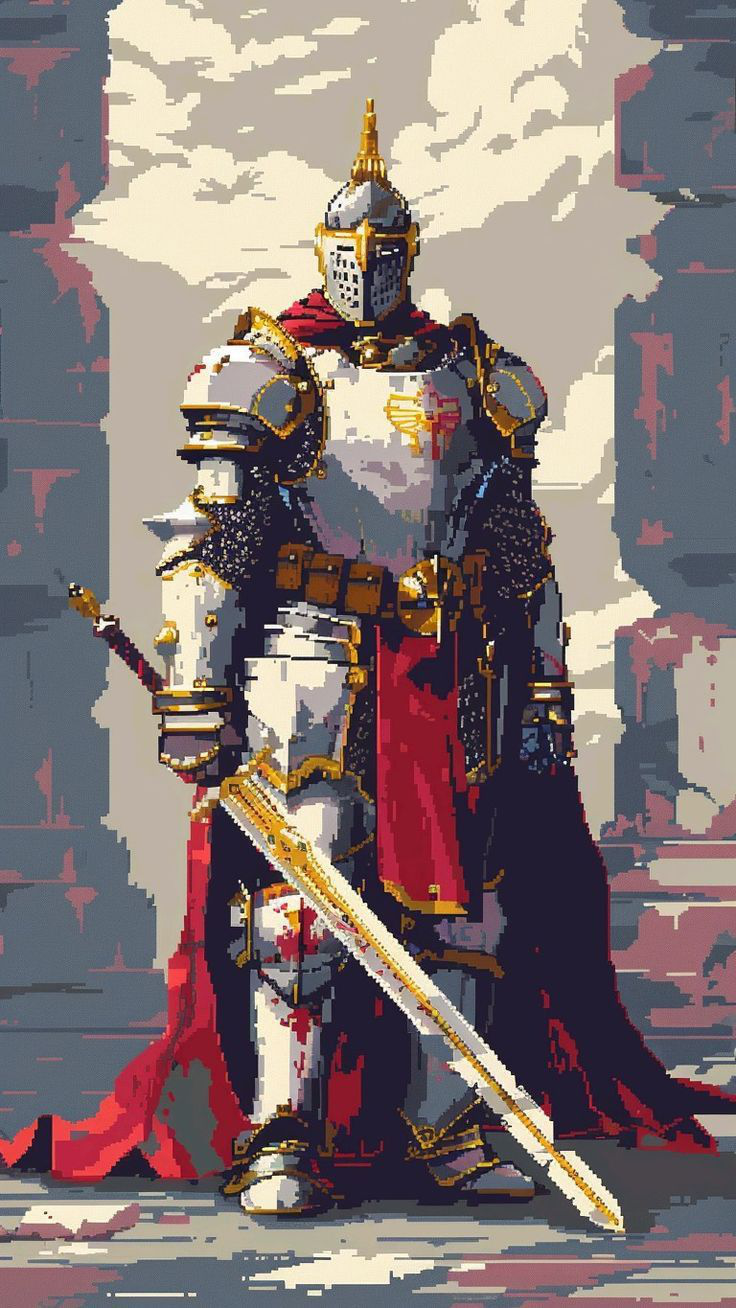
\includegraphics[width=0.8\linewidth]{img2.png} \\Концепт мечника со шпагой}
\end{minipage}
\hfill
\begin{minipage}[h]{0.49\linewidth}
\center{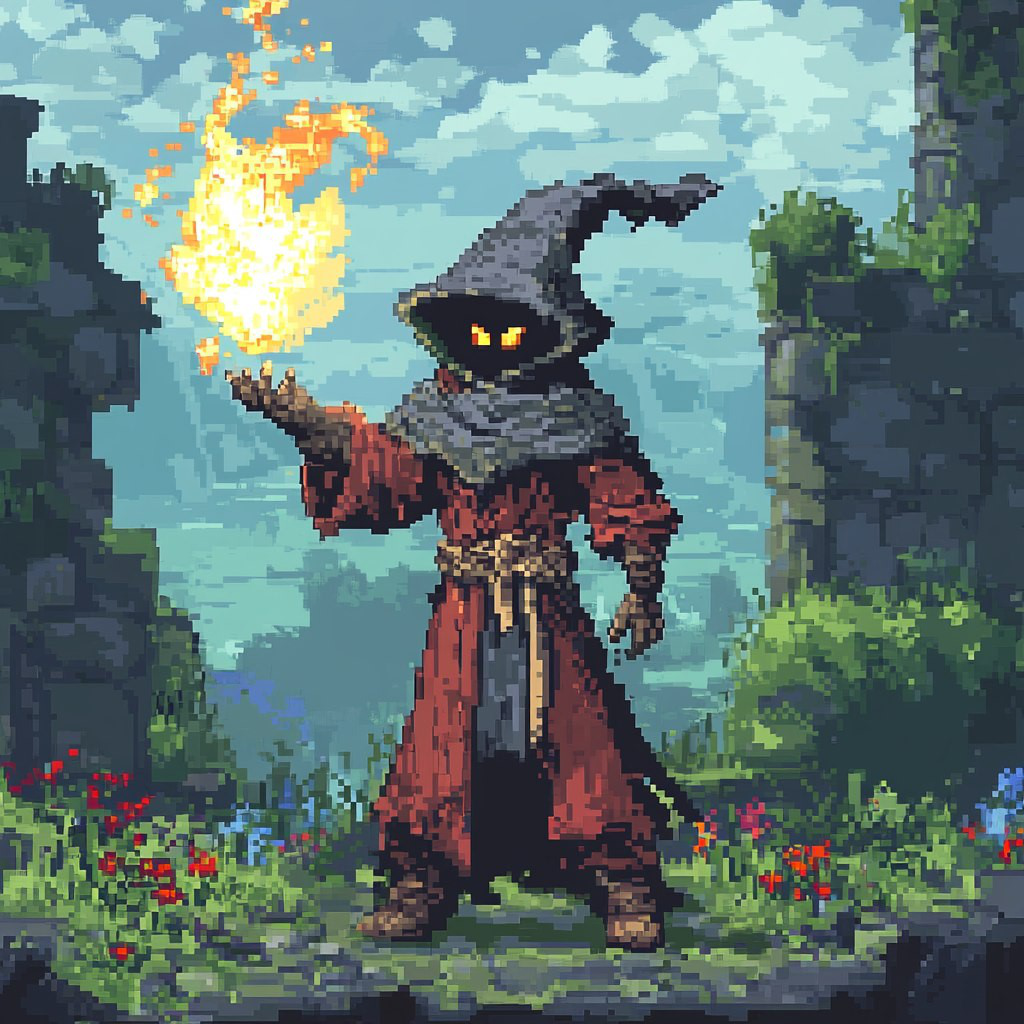
\includegraphics[width=0.8\linewidth]{img4.png} \\  Концепт мага с книгой}
\end{minipage}
\caption{Предварительные концепты}
\label{ris:image1}
\end{figure}

\begin{figure}[H]
\begin{minipage}[h]{0.49\linewidth}
\center{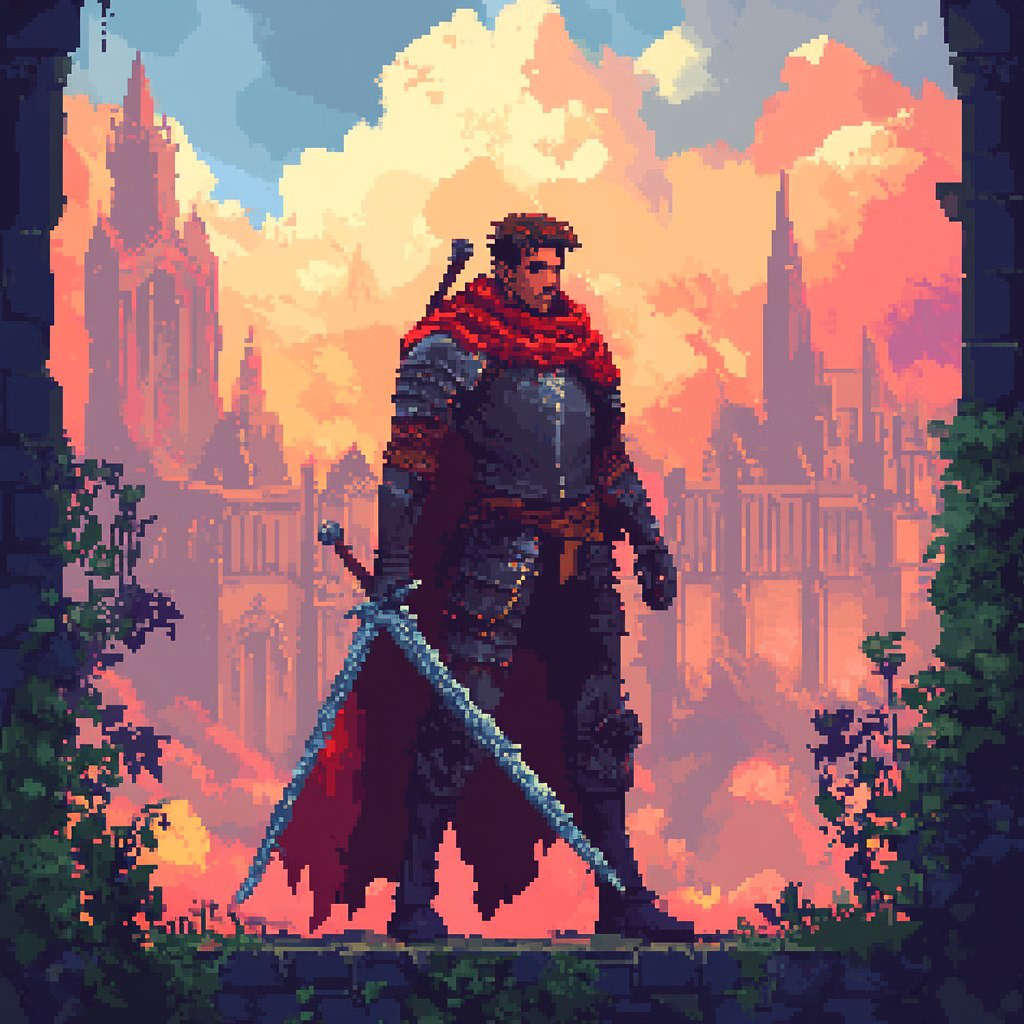
\includegraphics[width=0.8\linewidth]{img.png} \\Концепт мечника с двуручным мечом}
\end{minipage}
\hfill
\begin{minipage}[h]{0.49\linewidth}
\center{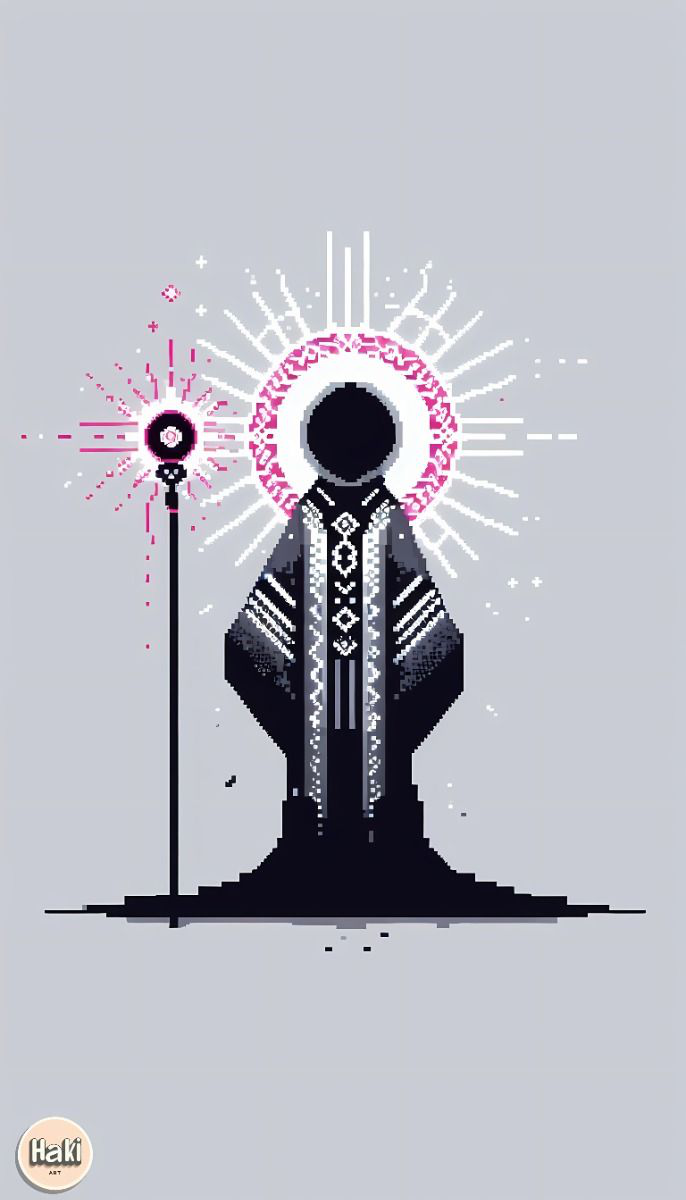
\includegraphics[width=0.8\linewidth]{img3.png}\\  Концепт мага с магическим посохом}
\end{minipage}
\caption{Предварительные концепты}
\label{ris:image1}
\end{figure}

Имя персонажа даётся игроком в начале игры, так как персонаж в начале сюжета не имеет никаких воспоминаний о прошлом себе. По мере развития сюжета игрок узнает о прошлом персонажа, его семье и близких из записок и писем.

\subsection{Элементы игры}
\subsubsection{Юниты и строения}
\par В игре представлено несколько основных локаций, в которых происходят действия игры. Приключение начинается в заброшенном замке. Это первое строение, с которым знакомится персонаж после сна. Замок поглощен таинственным туманом, вокруг – темные залы, освещенные факелами и разбросанные книги, и обрывки записок. По ходу исследования главный герой сталкивается с живыми скелетами, теневыми существами и различными ловушками. 
\begin{figure}
\begin{minipage}[h]{0.49\linewidth}
\center{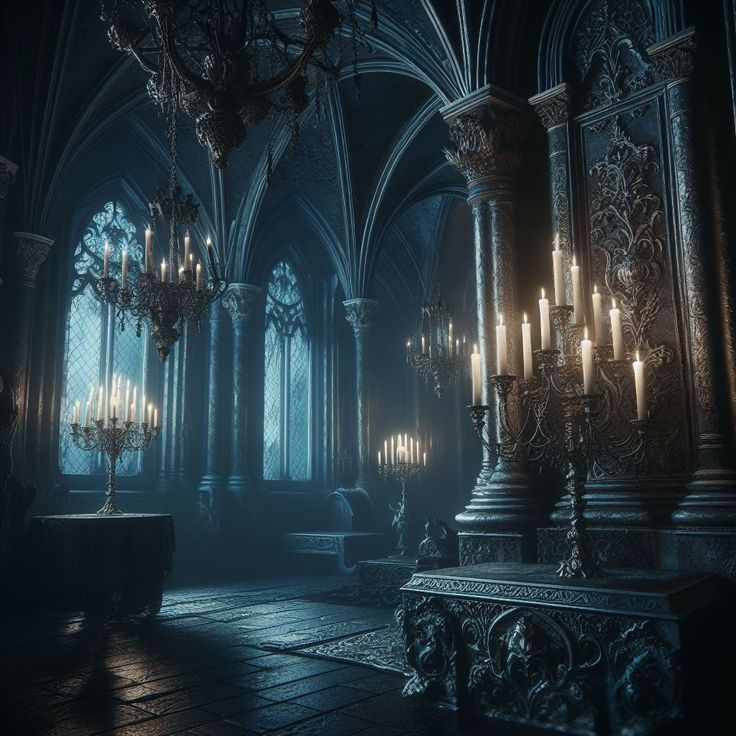
\includegraphics[width=0.8\linewidth]{image.png} \\рис.1 Локация 1 замок внутри}
\end{minipage}
\hfill
\begin{minipage}[h]{0.49\linewidth}
\center{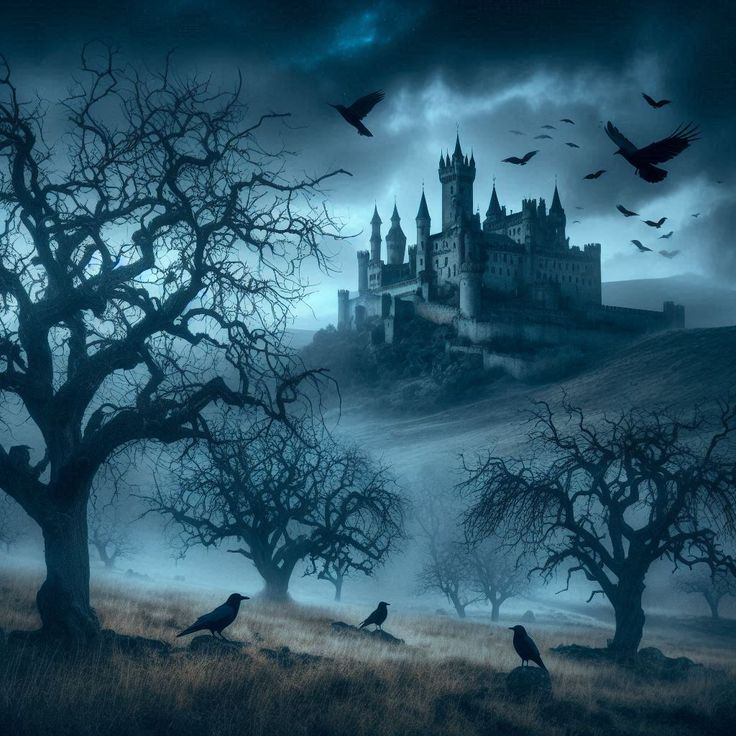
\includegraphics[width=0.8\linewidth]{image1.png} \\  рис.2 Локация 1 замок снаружи}
\end{minipage}
\end{figure}
\par Покинув замок, игрок сталкивается с загадочным незнакомцем, после он попадает в проклятый лес с часовой башней древнего оборотня.
Уже старая, но строго охраняемая башня находится среди деревьев. Она выглядит уже потрепанной, но часы еще идут.
\begin{figure}[h]
    \centering
    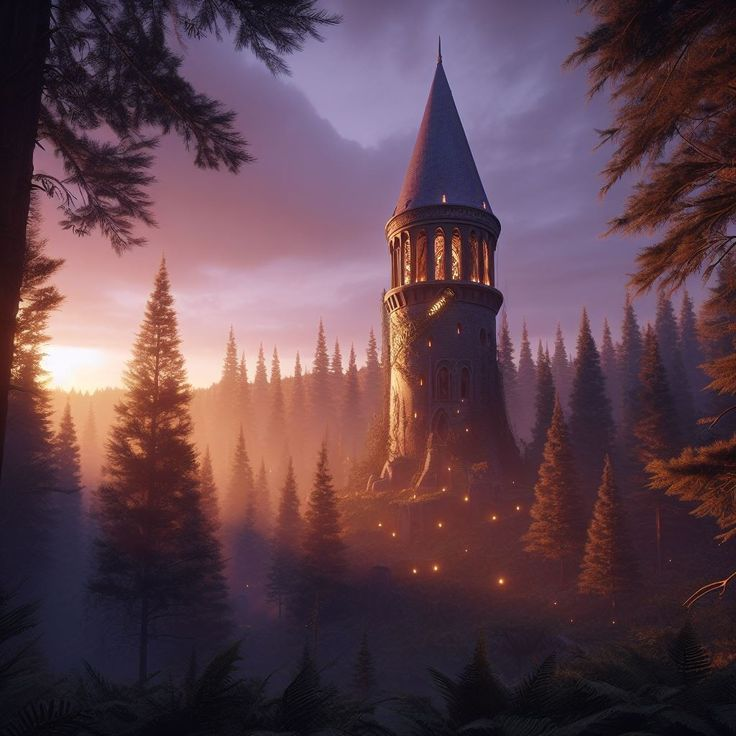
\includegraphics[width=0.5\linewidth]{image2.png} \\ рис.3 Часовая башня
    \label{fig:enter-label}
\end{figure}
\par Далее Подземелья замка, населенные духами, ожившими доспехами рыцарей и созданиями из плоти, порожденными Бездной. Игроку предстоит продвигаться через мрачные и узкие коридоры, сражаясь с противниками и разгадывая загадки.
\begin{figure}[h]
    \centering
    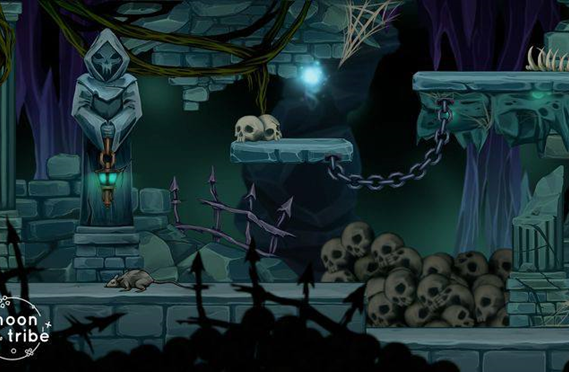
\includegraphics[width=0.5\linewidth]{image3.png} \\рис.4 Подземелья замка
    \label{fig:enter-label}
\end{figure}

\subsubsection{Предметы (items)}
\par Перейдем к такой же важно составляющей персонажа и атмосферы, как предметы. В игре есть один главный персонаж и его враги или помощники. Предметы можно разделить на категории: предметы главного персонажа, оружие (об этом подробнее далее в 3.4.3), предметы на локациях, предметы противников. 
\par Начнем с важной части нашей игры - записки. С помощью них герой узнает все о локациях, в записках описаны основные цели. Именно они помогают герою продвигаться. 
\begin{figure}[h]
    \centering
    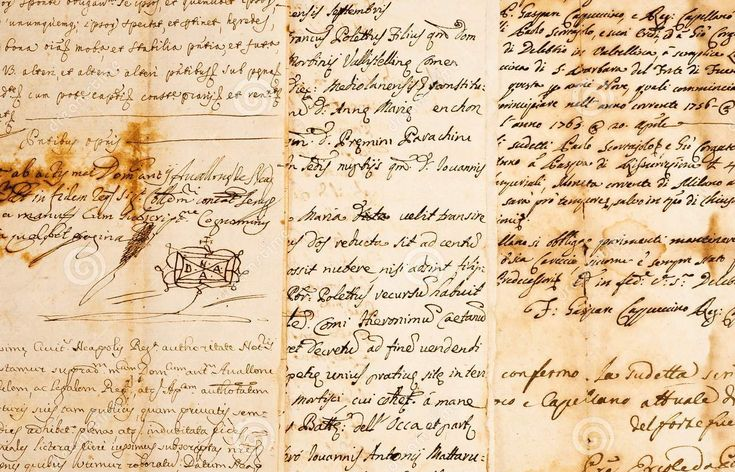
\includegraphics[width=0.5\linewidth]{image4.png} \\ рис.5 Записки
    \label{fig:enter-label}
\end{figure}
\par Безусловно далее стоит добавить информацию об основных предметах на локация. Это и старые книги в замках, и цепи вокруг, свечи и тому подобное. Все это создает атмосферу игры. 
\par Также важно частью игры несет артефакт, части которого герой собирает на протяжении игры. Это артефакт для подчинения мертвых, чтобы победить в финальном сражении. 
\begin{figure}[h]
    \centering
    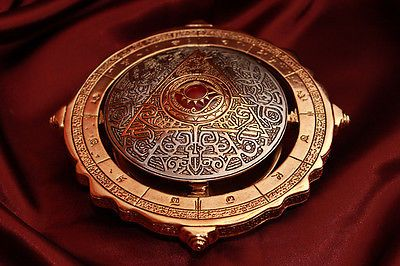
\includegraphics[width=0.5\linewidth]{image5.png} \\ рис.6 Артефакт
    \label{fig:enter-label}
\end{figure} 
\par В процессе игрок получает и другие полезные предметы, которые будут ему помогать (зелья, рецепты и заклинания, кристаллы силы). В локациях в разных местах будут находиться сундуки, где можно найти ключи для запертых дверей, монеты, зелья (хил, скорость, сила), различные предметы (например, ботинки-скороходы, увеличивающие скорость передвижения, цепкие перчатки для лазания по стенам, крылья для полета на некоторое время) и т.д. За монеты можно будет покупать оружие и броню у торговцев, а также прокачивать их. 
\subsubsection{Оружие}
\par Оружие в целом можно разделить на два вида: оружие главного героя и оружие врагов. Что касается злодеев, это разнообразные магические приспособления, заклинания. Они защищены броней и носят специальные костюмы. 
\par Что касается главного персонажа, артефакт также является оружием для борьбы с главным злодеем. Его поиском герой занимается всю игры (рис.6). Также это специальные костюмы, щит, меч и броня, также магический посох. Все это можно увидеть на картинках вида главного героя. 
Безусловно есть и другое вспомогательное оружие, которое герой покупает всю игру. Это мощные заклинания, броня для усиления атаки и тому подобное.
\subsubsection{NPC и персонажи}
Как мы и писали ранее у нас есть два варианта игровых персонажей: мечник и маг, у каждого из них есть свои особенности (см. пункт 3.3). В этом же разделе больше расскажем про персонажей NPC. Для каждый зоны свои персонажи: например, для Заброшенного замка это скелеты и тени. Они не слишком сложные для прохождения,ибо игрок только учится использовать  базовые атаки и уклонения.\par
Следующий персонаж - Незнакомец, он не играбельный, однако достаточно влиятельный в контексте самой игры и ее сюжета. Он является катализатором начала игры, а так же задает направление пути героя. Незнакомец выглядит как старый изгой отшельник, но по его манере речи и некоторым деталям его одежды(кольцо, компас и шляпа), герой понимает, что старик не такой уж и простой и относится к нему как  к мудрецу, знающий больше чем любой человек в этом мире. После встречи с Незнакомцем герой переходит на новый уровень где встречает других NPC -  волков и пауков. Они немного сильнее чем скелеты и тени, и волки наносят урона больше чем пауки. \par
Первый важный босс - Древний Оборотень: это персонаж, который больше главного героя в 2-3 раза, однако не смотря на размере бьет он достаточно средне(в сравнении с остальными боссами). Босс служит больше устрашением визуальным из-за его большого размера, в добавок у него красные глаза и броня на жесткая синяя шерсть, которая не пропускает почти ни одной пули/удара/магического воздействия. \par
Следующая локация: Скалы Пепельного Крика. Там герой сталкивается с усиленными тенями(духами) из первой сцены, они больше по размеру и в отличие от теней, духи наносят намного больше урона, а также у них есть очертания их прошлых человеческих обличий. Босс этого места - Тень
Некроманта: в черном обличии, с косой, а также с ужасными дьявольскими отростками из его головы, которые прорываются из его капюшона. В его косе находится его магическая сила благодаря специальному кристалу, помещенному в нее.\par
Последний и самый главный босс - Хранитель Бездны. Он выглядит как рыцарь с железно-каменными крыльями, с рогами на его шлеме, фиолетовыми глазами, как его магическое пламя. Он также облачен в сверхпрочную броню с золотыми вставками и специальными кристаллами, защищающими его.
\subsubsection{Транспортные средства– simulators}
Что касается передвижения, в основном это просто пешком, так как суть игры - пешее приключение. Конечно, в игре так же можно прыгать, бегать, лазать, ибо это все облегчит прохождение уровней, а также увеличит манёвренность игрока. У некоторых предметов, а также у главного героя, в категории "маг" есть возможность левитации, но не на продолжительный срок, а на пару секунд. При переходя с одной локации на другую, будет работать "телепорт", где игрока просто переносят на другую локацию, в остальных же ситуациях телепорт работать не будет.\par

\subsubsection{Карты}
Вся карта будет делиться на 4 локации: Замок Тьмы, Проклятый Лес, Скалы  Пепельного Крика, Подземелья Бездны. У каждого места своя атмосфера, своя цветовая палитра, свои особенные элементы, свое музыкальное сопровождение. \par
Замок Тьмы \par
Это стартовая локация, в которые игрок бродит по замку в поисках выхода, а также полезных вещей, соответственно карта похоже на планировку замка с некоторыми элементами лабиринта. В рамках отдельный комнаты же перемещение по ней идет горизонтально. Цветовая палитра замка имеет общий цвет - яркий зеленый, цвет который можно увидеть в заброшенных влажных местах, а так же акцентный цвет - синий/красный. Синий будет появляться в местах где видна улица, красный - только в закрытых помещениях. Сочетание этих цветов выглядит неприятно и некомфортно, поэтому идеально подойдет для странного заброшенного замка \par
Проклятый Лес \par
Изображен через теневые структуры, то есть мы видим достаточно яркий фон и контрастные деревья, ветки, лианы, отростки, корни. В цветовой палитре преобладают темное-зеленые цвета, а также немного сероватые светлые участки, показывающие туман. Карта будет горизонтальная, то есть пока вы идете, лес будет продолжаться. В конце вы найдете "выход" из этого проклятого места. \par
Скалы  Пепельного Крика \par
Эта локация будет выполнена в почти оттенках серого, однако некоторые цвета будут иметь холодные подтоны, не зависит от основного цвета(ощущение как будто вы убрали контрастность в картинки). Карта скал будет походить на нелинейный поход к/вокруг гор, чтобы достичь определенного подземелья в старом замке(не Замок Тьмы).  Весть путь будет разделен на части, в рамках которых передвижение будет линейным/горизонтальным.\par
Подземелья Бездны \par
Последняя локация для нашего героя будет исполнена в красноватых тонах, имитируя количество крови, которое здесь было пролито. Помимо этого светлые цвета будут так же яркими - оранжево-желтыми, они будут показывать "огонь", символизируй опасность. Так как это подземелье, то перемещение будет и горизонтальным и вертикальным, то есть мы можем как спуститься в низ, так и подняться повыше \par



\subsection{«Искусственный интеллект»}

\subsection{Многопользовательский режим}

\subsection{Интерфейс пользователя}

\subsubsection{Блок-схема}
\begin{figure}[h]
    \centering
    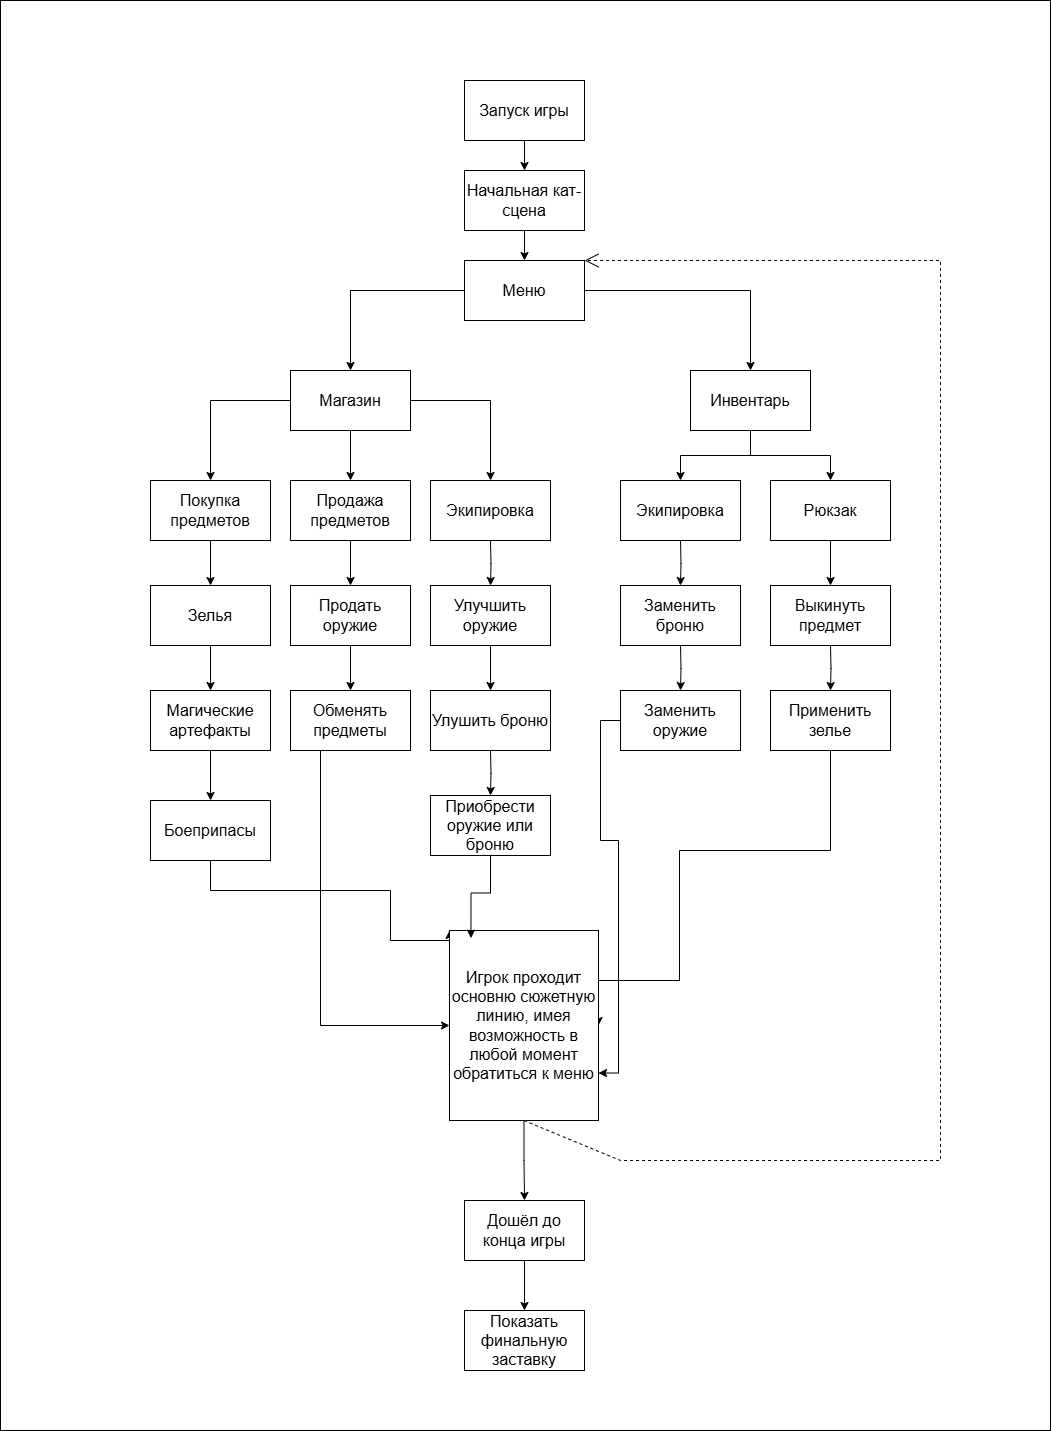
\includegraphics[width=370px\linewidth]{Интерфейс_диздок_(7.рис).png} \\ рис.7 Блок-схема навигации по меню игрового интерфейса
    \label{fig:artifact}
\end{figure}


\subsubsection{Функциональное описание и управление}
Игра начинается безусловно с начального экрана с кнопками старт, меню, настройки, фон и название, как и в любой игре. При нажатии на кнопку настройки игрок может контролировать громкость, масштаб, свое имя в игры и другое. При нажатии на кнопку меню у него появляется возможность выбрать себе класс: маг и мечник, их внешний вид. Есть информация о каждом. 
\par С нажатия кнопки старт начинается игровой процесс. Все начинается с истории героя, как он попадает в главный замок. Игрок не участвует в истории, а просто смотрит и читает информацию. Далее уже начинается игра и персонаж попадает в локации.
\par На основных локация, которые были описаны, герой может ходить, собирает полезные предметы. Также он встречается и борется с врагами. Есть возможность при достаточном количестве монет восстановить энергию или купить предметы в магазине или у торговцев. 
\par В игре будет присутствовать механика чек-поинтов и сохранений, вручную выполненный в виде привалов около костра, раскиданных по локациям. Данная механика позволит игрока вернутся в локацию, если она не полностью изучена или для поиска секретов.

\subsubsection{Объекты интерфейса пользователя}
На протяжении игры пользователь встретит следующие элементы интерфейса:
\begin{itemize}
\item[*] Классические кнопки: кнопка "Меню" в левом верхнем углу экрана; кнопка "Инвентарь"; кнопки навигации в инентаре "Магические артефакты", "Зелья", "Боеприпасы"; кнопка "Замена" для обновления экипированных предметов; кнопка "Читать" для писем и записок из инвентаря; кнопка "выкинуть" для удаления предметов из инвентаря; кнопка "Использовать" для зелий и артефактов; кнопки навигации в магазине "Купить", "Продать", "Улучшить"; кнопка "Выйти из игры";
\item[*] Чекбокс ("да или нет"): Подтверждение действия "Выбросить", "Заменить", "Использовать" в инвентаре; Подтверждение действия "Купить", "Продать", "Улучшить" в магазине.
\item[*] Слайдер: Выбор количество продаваемых или покупаемых единиц в магазине; Выбор количества зельев для использования; Настройки громкости внутриигровой музыки, звуков и эффектов. 
\item[*] Кнопки классические вблизи предметов с взаимодействием. Данные кнопки появляются, когда игрок находиться рядом с торговцем, костром для сохранения, сундуками, ресурсами, надписями на стенах. Визуально отображаются над предметов, с которым возможно взаимодействие.
\item[*] Джойстик или стрелки для передвижения игрока в левом нижнем углу экрана.
\item[*] Кнопки для отдельных классов персонажей. Из-за особенностей каждого рода главного героя, умения и атака персонажа варьируется. Данные кнопки распалагаются в правом нижнем углу экрана, основной набор представляет собой "Уклонения", "Атака", "Блок".
\item[*] Кнопки триггер ивентов появляются внезапно при определенном событии в игре. Кнопка "Шок" появится в центре экрана с красной подсветкой. Необходимо прожимать эту кнопку для сохранения жизней персонажа,  например, когда он попадает в ловушку или глушен врагом.
\item[*] Иконка персонажа с отображением уровня здоровья, маны и золота. 
\end{itemize}

\subsection{Графика и видео}

\subsubsection{Общее описание}
Наша игра в 2D графике. Внешний вид персонажей, локации представлены выше. Прописана графика злодеев. У каждого есть свои супер силы (оживление демонов в помощь, тяжелые атаки, броня и много другое. 
\par Также в игре есть логика предметов. Игрок находит их, следит за появлением. Нахождение артефакта как раз является целью прохождения игры. Есть статические объекты, которые просто создают атмосферу (элементы интерьера, фоны, обычные предметы - ненужные герою).
\par Интерфейс достаточно понятный пользователю. Управление с помощью кнопок (классические кнопки, выбор героев и другое). Визуальные эффекты (подсветка, анимация, переходы), звуковые эффекты (нажатия кнопок, выбор героев), тактильная обратная связь (вибрация) и подтверждение выбора/результатов действий.


\subsubsection{Двумерная графика и анимация}

\textbf{Интерфейс}
Интерфейс игры выполнен в минималистичном пиксель-арт стиле, соответствующем общему визуальному оформлению игры. Основные элементы интерфейса включают:
\begin{itemize}
    \item Панель здоровья и маны, отображающую текущие параметры персонажа.
    \item Индикаторы опыта и уровня для отслеживания прогресса прокачки.
    \item Быстрый доступ к инвентарю (зелья, оружие, предметы).
    \item Карта или указатели, помогающие ориентироваться в локациях.
    \item Подсказки и уведомления (например, о нахождении ключей или сундуков).
\end{itemize}

Анимация интерфейса включает:
\begin{itemize}
    \item Плавные переходы между экранами.
    \item Подсветку активных элементов.
    \item Визуальные эффекты подтверждения действий (например, мигание или небольшое увеличение кнопки при выборе).
\end{itemize}

\textbf{Эффекты}

Для создания атмосферы средневекового дарк-фэнтези в игре используются следующие визуальные эффекты:
\begin{itemize}
    \item Анимации атак (вспышки, следы от удара меча, магические заклинания).
    \item Эффекты освещения, такие как мерцание факелов, свет от заклинаний или сияние артефактов.
    \item Частицы: падающая пыль в подземельях, искры от ударов, капли крови или дождя.
    \item Анимации разрушения объектов (например, разбивание ящиков или открытие сундуков).
\end{itemize}

\textbf{Основная игровая графика. Персонажи}

\begin{itemize}
    \item Главные герои (мечник и маг) имеют уникальные спрайты с анимациями ходьбы, атак, получения урона и использования предметов.
    \item Противники варьируются по внешнему виду и размерам: от обычных монстров до боссов с детализированными анимациями (например, оживление демонов, тяжелые удары или использование магии).
\end{itemize}

\textbf{Основная игровая графика. Игровой мир}

\begin{itemize}
    \item Локации включают замки, подземелья и открытые пространства, выполненные в пиксель-арт стиле с высокой детализацией текстур.
    \item Ландшафты содержат статические объекты: стены с трещинами, факелы, мебель, обломки и другие элементы интерьера для создания атмосферы.
    \item Взаимодействуемые объекты (сундуки, двери, рычаги) имеют выделяющиеся визуальные эффекты для привлечения внимания игрока.
\end{itemize}

\textbf{Анимация}

Каждый объект в игре имеет анимацию для усиления погружения:
\begin{itemize}
    \item Движение персонажей и врагов проработано через циклы ходьбы, бега и атак.
    \item Открытие сундуков сопровождается плавной анимацией крышки и вспышкой света.
    \item Магические заклинания включают анимацию зарядки, выпуска и попадания.
\end{itemize}

Общий стиль графики выдержан в духе тёмного средневекового фэнтези с использованием ограниченной палитры цветов (тёмные оттенки с акцентами ярких деталей).
 

\subsubsection{Трехмерная графика и анимация}

\subsubsection{Анимационные вставки}
Перечень и расположение анимационных вставок в игре\par
\begin{itemize}
    \item \textbf{Интро:}  
    \begin{itemize}
        \item \textbf{Местоположение:}  Местоположение: В начале игры, перед началом игрового процесса.\par
        \item \textbf{Характер исполнения:} Отдельная анимация, с выполнением в художественном стиле, не сильно отличном от игрового, но также сохраняется стиль "пикселизации", как и в игре.\par
        \item \textbf{Содержание:} Показывает, как главный герой открывает глаза, тем самым просыпается в пустом замке, пытается понять где он, идет небольшой монолог с его мыслями, о том что же ему делать дальше. Дальше он выходит из зала и сталкивается с темными силуэтами в тумане.  остальную же часть до нахождения записки ему надо пройти самому.\par
        \item \textbf{Продолжительность:} 1-2 минуты.\par
  \end{itemize}
    \item \textbf{Ролик при нахождении записки:} 
     \begin{itemize}
        \item \textbf{Местоположение:}  При нахождении каждой ключевой записки в игре. \par
        \item \textbf{Характер исполнения:} На «движке» игры, с анимацией открытия и плавным переходом к тексту.\par
        \item \textbf{Содержание:} Анимация того как герой, поднимает записку и раскрывает ее, потом его реакция на прочитанное. Затем переход к её содержимому, сопровождающееся визуальными эффектами, отражающими атмосферу.\par
        \item \textbf{Продолжительность:}  10-20 секунд.\par
  \end{itemize}
\item \textbf{Ролики с введением перед каждой главой игры:} 
    \begin{itemize}
        \item \textbf{Местоположение:} В начале каждой из четырех ключевых локаций.\par
        \item \textbf{Характер исполнения:} Отдельные анимации, выполненные в том же художественном стиле, что и начальный ролик.\par
        \item \textbf{Содержание:} Краткое введение в задачу миссии, показывающее. Эти ролики могут содержать очень краткий обзор событий, приводящих к текущему заданию. В основном в ролике будет краткий обзор на локацию(визуально), дабы не спойлерить игроку миссию. \par
        \item \textbf{Продолжительность:} 15-25 секунд.\par
  \end{itemize}

  \item \textbf{Ролик финальной битвы в каждой главе:} 
   \begin{itemize}
        \item \textbf{Местоположение:} Перед сражением с боссом.\par
        \item \textbf{Характер исполнения:}Отдельная анимация, выполненная с высоким качеством концепции аудио и визуальными эффектами для создания напряженной атмосферы.\par
        \item \textbf{Содержание:} Показано, как основной появляется, возможно, мини-диалог, но в основном - враг готовится к бою, пробуждая свои темные силы/настраивая свои клинки и тд. В игрока вселяется ужас, а также страх предстоящей битвы .\par
         \item \textbf{Продолжительность:} 1-2 минуты.\par
\end{itemize}  
\item \textbf{Аутро:} 
    \begin{itemize}
        \item \textbf{Местоположение:} После завершения игры, по окончании финальной битвы с последним боссом.\par
         \item \textbf{Характер исполнения:} Отдельная анимация, с завершением в стилистике игры.\par
        \item \textbf{Содержание:} Показано, как светнемного возвращается в мир, освещая картинку и сцену, после победы игрока. Главный герой все еще пытается вспомнить что же произошло на самом деле, исходя из всех собранных записок. Но при этом дается намек на новые вызовы, ибо После встречи с Незнакомцем игрок понимает, что не все правда раскрыта, зло еще есть и с этим придется столкнуться в последующих частях игры.\par
        \item \textbf{Продолжительность:} 1-2 минуты.\par
  
\end{itemize}  
\end{itemize}
\begin{itemize}
\item \textbf{Характер исполнения:}
    \begin{itemize}
        \item \textbf{}Все ролики, кроме вставок при нахождении записок, являются отдельными анимациями, что позволяет создать более выразительные визуальные и звуковые эффекты, которые подчёркивают атмосферу и напряжение игры.
        \item \textbf{}Вставки с записками реализованы на «движке» игры, чтобы сохранить непрерывность игрового процесса.
    \end{itemize}
\item \textbf{Содержание:}
    \begin{itemize}
        \item \textbf{}Начальный ролик задает тон, вводя игрока в мрачный и таинственный мир, исследование которого станет основной задачей. 
        \item \textbf{}Ролики в начале локаций и ролики с нахождением записок погружают игрока в сюжет, делая акцент на прогресс игрока, подчеркивая важные события и направления.
        \item \textbf{}Ролики финальных битв, дают время игроку на мобилизацию всех его ресурсов для успешного прохождения грядущего испытания “на прочность”.

        \item \textbf{}Финальный ролик подводит итог приключению и дарит игроку ощущение завершенности, показывая последствия его действий.
    \end{itemize}
\end{itemize}
\subsection{Звуки и музыка}

\subsubsection{Общее описание}

\subsubsection{Звук и звуковые эффекты}

\subsubsection{Музыка}

\subsection{Описание уровней}

\subsubsection{Общее описание дизайна уровней}

\subsubsection{Диаграмма взаимного расположения уровней}

\subsubsection{График введения новых объектов}

\section{Контакты}

\newpage

\title 

\end{document}
